% Istanbul Arel University thesis template, adapted for the WashFlow midterm.
\documentclass[12pt]{report}
\usepackage{arel_thesis}
\usepackage[top=1cm,bottom=2.54cm,left=3.17cm,right=3.17cm]{geometry}
\usepackage{booktabs}
\usepackage{pdflscape}
\usepackage{tikz}
\usetikzlibrary{arrows.meta}
\usepackage[hidelinks]{hyperref}
\hypersetup{pdftitle={WashFlow Midterm Thesis Progress Report}}

\degree{Bachelor of Science}
\department{Computer Engineering}
\gradyear{November 2026}
\studentname{Barış Gündoğdu}
\studentid{230303912}
\supervisor{Dr. Tuğberk Kocatekin}
\title{WashFlow\\Midterm Thesis Progress Report}
\trtitle{WashFlow\\Mezuniyet Projesi Ara Raporu}
\renewcommand{\bibname}{References}
\setlength{\emergencystretch}{2em}

\newcommand{\capturepanel}[3]{%
  \begin{minipage}[t]{.47\linewidth}\centering
    \textbf{#2}\par\medskip
    \IfFileExists{screenshots/#1.png}{%
      \includegraphics[width=.96\linewidth,height=.52\textheight,keepaspectratio]{screenshots/#1.png}\par
    }{%
      \fbox{\parbox[c][.26\textheight][c]{.86\linewidth}{\centering
        \textit{Screenshot pending}\par\smallskip\small #3}}\par
    }%
  \end{minipage}%
}

\begin{document}
\setstretch{1.5}
\hypersetup{pageanchor=false}
\maketitle
\hypersetup{pageanchor=true}

\begin{preliminary}
\chapter*{Acknowledgement}
I would like to express my sincere gratitude to my supervisor, Dr. Tuğberk Kocatekin, for his guidance and valuable feedback throughout the development of this graduation project.

I would also like to thank the faculty members of the Computer Engineering Department at Istanbul Arel University for the knowledge and support they have provided during my undergraduate education.

Finally, I am grateful to my family for their continuous encouragement and support throughout my studies.

\chapter*{Undertaking}
This is to declare that the project entitled ``WashFlow'' is an original work done by undersigned, in partial fulfillment of the requirements for the degree ``Bachelor of Science in Computer Engineering'' at Computer Engineering Department, Faculty of Engineering, Istanbul Arel University.

All the analysis, design and system development have been accomplished by the undersigned. Moreover, this project has not been submitted to any other college or university.

\newpage
\begin{abstract}
WashFlow is a multi-tenant application under development for car wash businesses. Its midterm objective is to establish an operational workflow across a Flutter client, an ASP.NET Core Web API and PostgreSQL, with tenant authorization enforced by the server. The implementation supports role-aware authentication, employee invitations, owner management of local customer and vehicle records, and customer management of personally owned vehicles. It also provides business settings, service pricing and owner-managed appointment scheduling. The owner-side customer and vehicle workflow has documented simulator-to-database evidence from an isolated environment. The demo database was subsequently inspected in read-only mode and its schema matched a reference created from all seven Entity Framework Core migrations. The GitHub Actions run associated with pull request \#15 passed 398 backend tests and 341 Flutter tests. Employee work execution, customer self-service booking, walk-in queue management and financial reporting remain outside the completed scope.
\end{abstract}

\begin{ozet}
WashFlow, oto yıkama işletmeleri için geliştirilmekte olan çok kiracılı bir uygulamadır. Ara değerlendirme hedefi, Flutter istemcisi, ASP.NET Core Web API ve PostgreSQL arasında çalışan bir iş akışı kurmak ve işletme bazlı yetkilendirmeyi sunucuda uygulamaktır. Uygulama, role göre kimlik doğrulama ve gezinme, çalışan daveti, işletmeye ait müşteri ve araç kayıtları, müşterinin kendi araçlarını yönetmesi, işletme ayarları, hizmet fiyatlandırması ve işletme sahibinin randevu planlamasını destekler. Müşteri ve araç iş akışı, yalıtılmış bir ortamda iOS simülatöründen PostgreSQL'e kadar doğrulanmıştır. Demo veritabanının salt okunur incelemesinde şema, yedi Entity Framework Core geçişiyle oluşturulan referansla eşleşmiştir. GitHub Actions üzerinde 398 arka uç testi ve 341 Flutter testi başarılı olmuştur. Müşterinin kendi randevusunu oluşturması, çalışan iş akışları, sıra yönetimi ve finansal raporlama sonraki çalışma kapsamındadır.
\end{ozet}

\setstretch{1.0}
\tableofcontents
\listoffigures
\addcontentsline{toc}{chapter}{\listfigurename}
\listoftables
\addcontentsline{toc}{chapter}{\listtablename}
\end{preliminary}
\setstretch{1.5}

\chapter{Introduction}
WashFlow is a Computer Engineering graduation project for managing the operations of independent car wash businesses. It uses one mobile application for business owners, employees and customers. Each business constitutes a tenant, while customers may have platform accounts with their own vehicles. This report covers the midterm state of the demo branch at commit \texttt{cc346ac}, which includes the continuous integration workflow and the verified database diagram \cite{repo,ciPR,erdPR}. It describes implementation and verification completed to date.

\section{Problem Definition and Project Objectives}
The pilot business observations recorded in the requirements specification describe appointments taken by telephone, customer and vehicle history recorded inconsistently, and daily revenue and expenses tracked in notebooks. Busy periods make the allocation of staff and work areas harder to coordinate \cite{srs}. The project addresses this problem by keeping operational records in one system while enforcing clear boundaries between independent businesses.

The midterm objectives are to deliver one working owner workflow from the mobile interface to persistent storage, verify tenant isolation and scheduling rules in automated tests, and make the work reproducible through tracked migrations and CI. Later objectives include customer self-service booking and operational workflows beyond the appointment calendar.

\chapter{Background and Requirements Analysis}
The functional baseline is version 0.2 of the Software Requirements Specification \cite{srs}. It distinguishes business staff who act within a tenant from customers who own platform records. An owner can administer the business and its local customers, vehicles, service catalog and appointments. Employees enter through an invitation process and receive a restricted context. The customer context currently supports personally owned vehicles. This separation informs both route selection in Flutter and authorization decisions in the API.

The midterm vertical slice targets the owner-side milestone in the SRS. It requires identifying the current owner and business, creating a local customer, adding a vehicle under that customer and retrieving the saved records. Verification includes rejecting access by another business or an actor without the required role. Independently, a customer may manage their own vehicles. The SRS reserves verified linking of a local customer to a registered account for later work. Similar names or plates are insufficient evidence of identity.

Security and data consistency requirements include verified sign-in, scoped access to records, input validation and resistance to stale updates. Scheduling further requires checks for time, staff availability and work-area capacity, including competing requests. The application uses Turkish interface text for its intended operators. This report uses English with the Turkish summary provided by the university template.

\chapter{Method}
\section{System Architecture and Technology Stack}
Figure~\ref{fig:architecture} shows the runtime components of the implemented vertical slice. Flutter provides screens, controllers and API clients. The ASP.NET Core Web API groups endpoints by feature. The backend solution separates the API, application contracts and services, domain models, and infrastructure. Entity Framework Core and Npgsql map domain records to PostgreSQL. Migrations record changes to the schema and provide a reproducible baseline \cite{repo,efmigrations}.

\begin{figure}[htbp]
\centering
\setlength{\fboxsep}{8pt}
\fbox{\parbox{.81\linewidth}{\centering\textbf{Flutter mobile client}\\Owner context, customer form and vehicle list}}\\[4pt]
\(\downarrow\) \quad JSON request and bearer token \quad \(\uparrow\) response\\[4pt]
\fbox{\parbox{.81\linewidth}{\centering\textbf{ASP.NET Core Web API}\\Authentication, authorization, validation and application services}}\\[4pt]
\(\downarrow\) \quad EF Core / Npgsql \quad \(\uparrow\) persisted data\\[4pt]
\fbox{\parbox{.81\linewidth}{\centering\textbf{PostgreSQL}\\Tenant records, keys, constraints and migration history}}
\caption{Runtime components and request flow for the owner vertical slice.}
\label{fig:architecture}
\end{figure}

For protected operations, the API validates the JWT and evaluates the active session and the caller's access to the relevant scope. JWT defines the token format \cite{jwt}. WashFlow checks tenant membership and role against application data. The client uses the returned context to choose its navigation. For writes, server-side validation and database constraints cover cases in which a client sends stale or invalid values.

\section{Database Design and ER Diagram}
The schema separates \texttt{LocalCustomers} and \texttt{LocalVehicles}, which belong to a business, from \texttt{CustomerProfiles} and \texttt{OwnedVehicles}, which are associated with platform identities. Composite foreign keys in scheduling preserve tenant and ownership paths when an appointment references local customer, vehicle or resource records. PostgreSQL's \texttt{xmin} system column provides the row version used for optimistic concurrency on mutable records. The column inventory counts user-defined columns.

Figure~\ref{fig:erd-overview} shows selected physical relationships used by the owner workflow. Figure~\ref{fig:erd} in Appendix~\ref{app:erd} presents the complete verified schema. The audit confirmed the API connection target and extracted the live \path{washflow_phase9e_db} schema in a read-only transaction. The inventory contains 23 application tables and one EF migration history table, 219 columns including metadata, 38 foreign keys and seven applied migrations. The catalog matched the reference database built from the seven migrations. EF Core found no model changes relative to the latest migration snapshot. The separate \path{washflow_db} database had only the first two migrations \cite{schemaaudit,pgcatalogs}.

\begin{figure}[htbp]
\centering
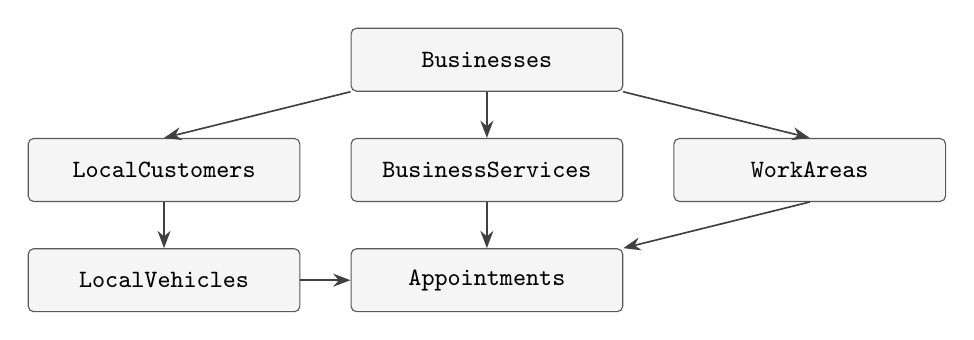
\begin{tikzpicture}[
  entity/.style={draw=black!65,fill=black!4,rounded corners=2pt,
    minimum width=3.45cm,minimum height=8mm,font=\small\ttfamily},
  relationship/.style={-{Stealth[length=2.2mm]},draw=black!75,semithick}]
  \node[entity] (business) at (0,2.8) {Businesses};
  \node[entity] (customers) at (-4.1,1.4) {LocalCustomers};
  \node[entity] (services) at (0,1.4) {BusinessServices};
  \node[entity] (areas) at (4.1,1.4) {WorkAreas};
  \node[entity] (vehicles) at (-4.1,0) {LocalVehicles};
  \node[entity] (appointments) at (0,0) {Appointments};
  \draw[relationship] (business.south west) -- (customers.north);
  \draw[relationship] (business.south) -- (services.north);
  \draw[relationship] (business.south east) -- (areas.north);
  \draw[relationship] (customers) -- (vehicles);
  \draw[relationship] (vehicles) -- (appointments);
  \draw[relationship] (services) -- (appointments);
  \draw[relationship] (areas.south) -- (appointments.north east);
\end{tikzpicture}
\caption[Selected foreign-key relationships for the owner workflow]{Selected foreign-key relationships for the owner workflow. Each arrow points from the referenced table to the referencing table. In each relationship shown, a parent row can have zero or more child rows, and each child row references one parent.}
\label{fig:erd-overview}
\end{figure}

\chapter{Results and Evaluation}
\section{Implementation Progress}
Table~\ref{tab:scope} distinguishes completed slices from capabilities that remain partial or planned. Here, completed refers to the stated slice and its available evidence.

\begin{table}[htbp]
\centering
\small
\begin{tabular}{@{}p{.22\linewidth}p{.70\linewidth}@{}}
\toprule
Status & Scope and evidence \\
\midrule
Completed & Owner and customer registration, email verification, sign-in and role-aware navigation. Owner invitation and employee acceptance. \\
Completed & Owner creation, search and editing of local customers and vehicles. Customers can manage vehicles belonging to their own account. Phase 7 records live simulator evidence for these data flows. \\
Completed & Business settings and weekly hours, service and vehicle-category pricing, and owner management of single-stage phone appointments with resource conflict checks. Scheduling has API, PostgreSQL and Flutter test coverage. \\
Partial & Employee access and scheduling availability exist. The employee interface does not yet provide work-order execution. Customer access covers personal vehicles, while profile editing and booking remain pending. \\
Planned & Public business discovery, customer self-service booking, walk-in queues, multi-stage work orders, payments, expenses and financial reports. \\
\bottomrule
\end{tabular}
\caption{Implementation scope at the midterm baseline.}
\label{tab:scope}
\end{table}

\subsection{Integrated owner vertical slice}
The owner selects the business context, enters customer details and submits them from Flutter. The client sends an authenticated request to the tenant-scoped customer endpoint. The API verifies the owner role, validates the input and calls the EF-backed store. The owner adds a vehicle through the nested customer endpoint, and the client retrieves the saved vehicle from the API. Database constraints and store queries enforce the relationship between business, customer and vehicle. The integration suite checks persistence and rejects foreign tenant identifiers and unauthorized actors \cite{repo,phase7}.

The Phase 7 record documents an isolated iOS simulator run against Kestrel and PostgreSQL. The owner created, searched and edited customer records and managed local vehicles. The harness established its authenticated session through the API adapter. The documented end-to-end run covers the customer and vehicle screens, with a sign-up rehearsal on the current build still pending \cite{phase7}.

\subsection{Scheduling decisions}
The owner can configure work areas, service requirements and employee availability. The scheduling API supports preview, creation, rescheduling and cancellation for owner-entered appointments. The preview gives the operator feedback before submission. The write path locks the business row in a PostgreSQL transaction and checks resource availability again because a competing request may have reserved the same resource in the meantime. This serializes scheduling writes within a business while allowing unrelated businesses to proceed independently. Availability and capacity checks use the active service interval, and the appointment keeps relevant price and duration values from the time of booking. Integration tests exercise simultaneous competing requests, version conflicts and repeated submissions \cite{phase9}. The repository evidence does not establish current on-device validation of the full scheduling flow.

\section{Testing and Continuous Integration}
CI runs on pushes and pull requests. The backend job uses .NET SDK 10.0.402, builds the solution in Release configuration and runs tests against a disposable PostgreSQL 17 service. The integration fixture creates and migrates isolated schemas in that service. The Flutter job uses Flutter 3.47.7, resolves dependencies from the lockfile, runs static analysis and executes the unit and widget test suite. Separate simulator tests provide evidence for the end-to-end database workflow \cite{fluttertesting,phase7}.

Table~\ref{tab:ci} reports the test counts from the PR \#15 job logs. The backend build passed, and the 398 backend tests include HTTP and PostgreSQL integration cases. Flutter static analysis reported no issues \cite{ciBackendLog,ciFlutterLog}.

\begin{table}[htbp]
\centering
\small
\begin{tabular}{@{}lrrr@{}}
\toprule
Suite & Passed & Failed & Skipped \\
\midrule
Backend unit tests & 252 & 0 & 0 \\
Backend integration tests & 146 & 0 & 0 \\
Flutter automated tests & 341 & 0 & --- \\
\bottomrule
\end{tabular}
\caption{GitHub Actions results for PR \#15. The Flutter completion line reports tests passed and gives no separate skip count.}
\label{tab:ci}
\end{table}

\section{Project Management and Development Methodology}
The work progressed from authentication and authorization to business settings, customer and vehicle management, service pricing and owner scheduling. This order established tenant identity and persistence before adding operations that depend on them. The repository uses GitHub Issues, a development board and pull requests to trace work. Issue \#12 and PR \#13 document CI. Issue \#14 and PR \#15 document the read-only database audit and ER diagram. Both PRs were merged into the demo branch \cite{ciPR,erdPR}. At the report baseline, 25 of the 39 commits reachable from that branch contained an issue reference in the commit message. This is below the 95\% target. Future changes should consistently link the corresponding issue.

\section{Current Limitations and Remaining Work}
The assessed deliverable is the owner customer and vehicle slice. Customer booking, walk-in queue management, employee execution of multi-stage jobs and financial reporting remain to be implemented. The current scheduler covers owner-entered appointments for a single service stage. Profile editing and verified linking between a business-local customer and a platform account also remain open. Pilot performance, usability and deployment have not been evaluated in this report.

Appendix~\ref{app:screens} documents the six application screens. The appointment image shows the empty agenda and provides evidence that the screen loads.

\chapter{Conclusion}
WashFlow has an implemented owner workflow that crosses Flutter, the ASP.NET Core API and PostgreSQL. The isolated simulator evidence demonstrates the customer and vehicle data flow, while the live catalog audit establishes the physical schema of the current demo database. Automated checks support reproducible verification of backend and Flutter changes. The next milestone extends this foundation to customer booking and operational workflows. Before the midterm demonstration, the current device build should be rehearsed from sign-up and email verification through customer and vehicle creation and retrieval after restart.

\cleardoublepage
\phantomsection
\addcontentsline{toc}{chapter}{\bibname}
\bibliographystyle{IEEEtran}
{\raggedright\bibliography{references}}

\appendix
\clearpage
\newgeometry{margin=1.35cm}
\begin{landscape}
\chapter{Complete Verified PostgreSQL ER Diagram}
\label{app:erd}
\vspace{-0.65cm}
\begin{figure}[h!]
\centering
\includegraphics[width=\linewidth,height=.70\textwidth,keepaspectratio]{figures/live-erd.pdf}
\caption[Complete verified PostgreSQL ER diagram]{Complete schema of \texttt{washflow\_phase9e\_db}. The diagram distinguishes EF migration history from application tables. The vector drawing can be enlarged for column and key labels.}
\label{fig:erd}
\end{figure}
\end{landscape}
\restoregeometry

\chapter{Application Screenshot Evidence}
\label{app:screens}
The captures show the Flutter app on an iPhone 18 Pro simulator. The owner workflow used the ASP.NET Core API and a disposable PostgreSQL instance populated with synthetic records. Figures~\ref{fig:auth-captures}, \ref{fig:owner-captures}, and~\ref{fig:vehicle-schedule-captures} show the captured screens.
\begin{figure}[h!]
\centering
\capturepanel{01-sign-in}{Sign in}{Open \emph{Giriş yap} from the welcome screen.}
\hfill
\capturepanel{02-sign-up}{Owner sign-up}{Open \emph{Kayıt ol} and choose \emph{İşletme kaydı}.}
\caption{Authentication screens.}
\label{fig:auth-captures}
\end{figure}
\clearpage
\begin{figure}[h!]
\centering
\capturepanel{03-owner-dashboard}{Owner dashboard}{Sign in with a synthetic owner account and open its business context.}
\hfill
\capturepanel{04-customer-management}{Customer management}{Open \emph{Müşteriler ve araçlar} and show the synthetic customer list.}
\caption{Owner navigation and business-local customer management.}
\label{fig:owner-captures}
\end{figure}
\clearpage
\begin{figure}[h!]
\centering
\capturepanel{05-vehicle-management}{Vehicle management}{Open the synthetic customer record and show its saved vehicle.}
\hfill
\capturepanel{06-appointment-scheduling}{Appointment scheduling}{Open \emph{Planlama ve randevular} and show the calendar.}
\caption{A saved synthetic vehicle and the owner appointment calendar in its empty state.}
\label{fig:vehicle-schedule-captures}
\end{figure}
\end{document}
